\documentclass[10pt]{article}
\usepackage[margin=0.72in]{geometry}
\usepackage{amsmath,amssymb,booktabs,array,graphicx,xcolor,hyperref,xurl}
\usepackage{microtype}
\hypersetup{colorlinks=true,linkcolor=blue,urlcolor=blue}
\newcommand{\ii}{\mathrm{i}}
\title{EDMD audit of relaxation modes in the controlled three-mode NLS system}
\author{Numerical validation report}
\date{7 September 2026}

\begin{document}
\maketitle

\begin{abstract}
We applied Extended Dynamic Mode Decomposition (EDMD) to four existing,
projection-free Cartesian trajectory ensembles for the three-mode chain.  The
state could be reconstructed from every stored snapshot, so no new dynamics
were simulated.  The constant mode, Gram conditioning, cutoff sensitivity,
dictionary, lag, timestep, and whole-trajectory bootstrap checks were fixed
before spectra were inspected.  In the driven system only one nontrivial rate
passes every gate, $\lambda\simeq-0.95$.  Two faster candidates cannot be
statistically separated, and the known oscillation near
$\operatorname{Im}\lambda\simeq5.3$ fails lag convergence.  The calculation
therefore does not establish several distinct driven slow modes.  It supports
one common leading mode with observable-dependent contamination from unresolved
faster modes.  At equilibrium, real rates near $-0.95$ and $-2.85$ pass all
gates at both timesteps.
\end{abstract}

\section{Question and data}
The controlled autocorrelation study found, at the fine timestep in the driven
case, plateau rates $-0.9351$ for $I_2$, $-1.0028$ for $I_1+I_3$, $-1.0921$
for $\cos\theta_3$, and $-1.1218$ for
$\cos\theta_1+\cos\theta_3$.  EDMD asks whether these are mixtures of several
generator modes rather than estimates of one unresolved gap.

The input consists of 64 independent trajectories for each bath condition
$(T_1,T_3)=(2,8)$ and $(5,5)$ and each integration timestep
$10^{-3}$ and $2.5\times10^{-4}$.  Each trajectory has burn-in 500,
stationary duration 1000, and 100001 snapshots at spacing 0.01.  The simulator
used double-precision state, a fixed timestep, standard trigonometry, and no
action floor or projection; snapshots were written as float32 observables.

No rerun was required.  The full reduced state is algebraically reconstructed:
\[
I_1=\tfrac12[(I_1+I_3)+(I_1-I_3)],\quad
I_3=\tfrac12[(I_1+I_3)-(I_1-I_3)],
\]
with $I_2$ saved directly and
$\theta_r=\operatorname{atan2}(\sin\theta_r,\cos\theta_r)$.

\section{Frozen EDMD estimator}
Actions use standardized logarithms
$z_j=(\log\max(I_j,10^{-12})-\overline{\log I_j})/s_j$.
Action monomials have total degree at most $d$.  The angular factor is the real
Fourier basis on the two-torus with $|m_1|,|m_3|\le M$.  Their tensor product
gives dictionaries D1 $(d,M)=(2,1)$, D2 $(2,2)$, and D3 $(3,2)$, with
$K=90,250,500$ respectively; the constant is always included.

Each stream contributes 2048 fixed, evenly spaced origins, giving 131072 pairs
per case.  At lags $\tau=0.10,0.25,0.50,1.00$ we estimate
\[
A_{ij}=\langle\psi_i(X_s)\psi_j(X_s)\rangle,\qquad
B_{ij}=\langle\psi_i(X_s)\psi_j(X_{s+\tau})\rangle,
\quad K_\tau=A^+B.
\]
The primary Gram-eigenvalue cutoff is $10^{-10}$ relative to the largest
eigenvalue, with fixed sensitivity checks at $10^{-8}$ and $10^{-12}$.
Rates use the principal logarithm $\lambda=\log\mu/\tau$.  Uncertainty is from
500 resamples of the 64 complete trajectories.

The complete predeclared gates are in \texttt{PROTOCOL.md}.  Briefly, a mode
must be stable across all three dictionaries, all four lags, and both
timesteps; have at least 90\% successful bootstrap matches; and have a
real-part interval separated from neighbouring reportable candidates.

\section{Mandatory convergence checks}
\subsection{Trivial mode, conditioning, and cutoff}
All full-sample fits recover the constant eigenfunction with
$|\mu-1|<1.2\times10^{-14}$.  D3 retains all 500 Gram directions.  Its
condition number ranges from $4.27\times10^3$ to $1.41\times10^4$ across the
four datasets.  Because the smallest retained direction remains above
$10^{-8}$ of the largest, all three fixed cutoffs retain the same 500
directions and give identical printed spectra.  These controls pass.

\subsection{Leading-rate convergence}
Table~\ref{tab:slow} gives the leading nontrivial rate before combining all
gates.  The D1--D3 drift is appreciable but lies inside the frozen 20\%
tolerance; lag and timestep gates also pass.

\begin{table}[h]
\centering\small
\caption{Leading nontrivial real rate.  Brackets are 95\% whole-stream
bootstrap intervals for D3 at $\tau=0.5$.}
\label{tab:slow}
\begin{tabular}{@{}lrrrr@{}}
\toprule
case & D1 & D2 & D3 [95\% CI] & D3 lags $0.1\to1.0$\\
\midrule
driven, $10^{-3}$ & -1.1053 & -1.0904 & -0.9402 [-0.9546,-0.9208] & -0.9779,-0.9619,-0.9402,-0.9218\\
driven, $2.5\,10^{-4}$ & -1.1250 & -1.1118 & -0.9632 [-0.9800,-0.9419] & -1.0558,-0.9870,-0.9632,-0.9451\\
equil., $10^{-3}$ & -1.1357 & -1.1232 & -0.9551 [-0.9724,-0.9328] & -1.0718,-1.0164,-0.9551,-0.9335\\
equil., $2.5\,10^{-4}$ & -1.1121 & -1.0980 & -0.9408 [-0.9548,-0.9230] & -1.0518,-0.9748,-0.9408,-0.9212\\
\bottomrule
\end{tabular}
\end{table}

\begin{figure}[h]
\centering
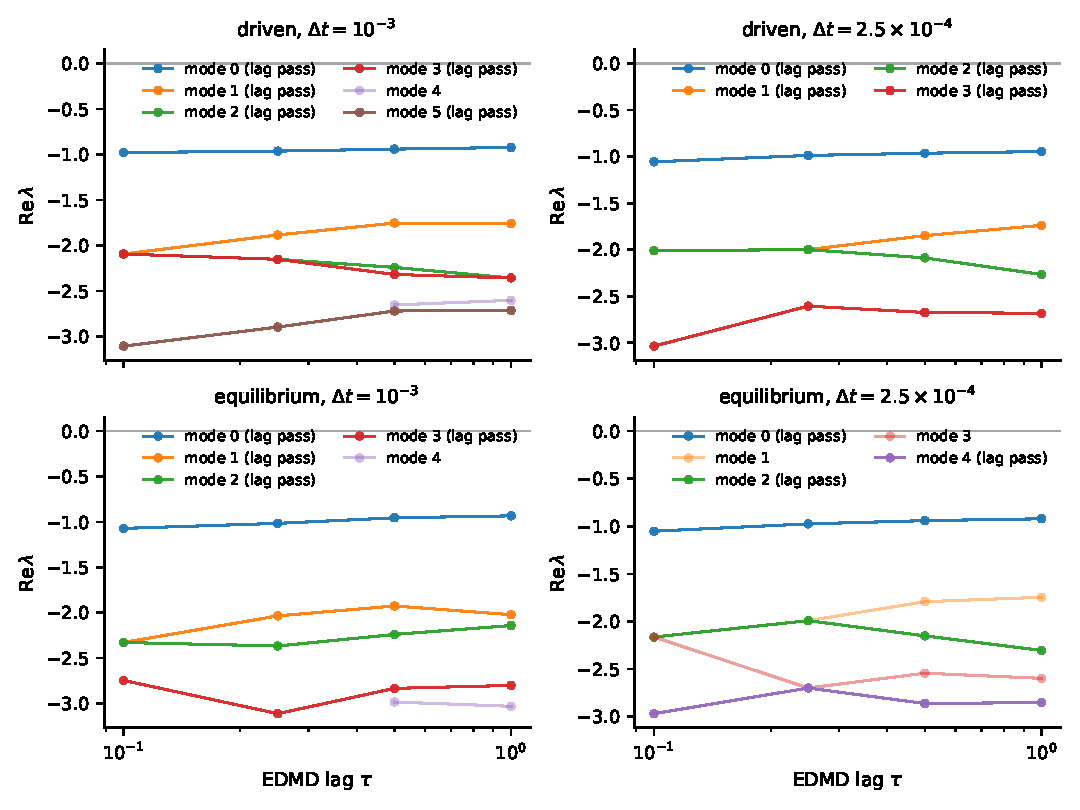
\includegraphics[width=.92\linewidth]{../figures/edmd_lag_convergence.pdf}
\caption{Raw lag dependence of the first frozen reference candidates.  Faded
curves fail that candidate's lag gate; a lag pass alone does not imply final
reportability.}
\end{figure}

\subsection{Modes that survive every gate}
\begin{table}[h]
\centering\small
\caption{Final reportable modes.  Rates absent from this table remain in the
raw spectra and failed at least one frozen gate.}
\begin{tabular}{@{}llrrr@{}}
\toprule
bath & timestep & $\operatorname{Re}\lambda$ & 95\% CI & $\operatorname{Im}\lambda$\\
\midrule
driven & $10^{-3}$ & -0.940174 & [-0.954628,-0.920824] & 0\\
driven & $2.5\,10^{-4}$ & -0.963191 & [-0.980007,-0.941942] & 0\\
equilibrium & $10^{-3}$ & -0.955149 & [-0.972388,-0.932803] & 0\\
equilibrium & $2.5\,10^{-4}$ & -0.940758 & [-0.954830,-0.922965] & 0\\
equilibrium & $10^{-3}$ & -2.833818 & [-2.946075,-2.705420] & 0\\
equilibrium & $2.5\,10^{-4}$ & -2.862538 & [-2.931237,-2.741557] & 0\\
\bottomrule
\end{tabular}
\end{table}

The driven candidates near $-1.8$ and $-2.1$ each pass the point-estimate
dictionary/lag/timestep tolerances but fail separation: at the fine timestep
their intervals are $[-1.991,-1.701]$ and $[-2.303,-1.779]$, which overlap.
At the coarse timestep the corresponding intervals are
$[-1.971,-1.533]$ and $[-2.542,-1.895]$.  They cannot be claimed as two
resolved eigenvalues.

\subsection{Known oscillatory control}
At $\tau=0.5$, a complex candidate can be found with imaginary part close to
5.3 in every dataset.  However, its real part and, at long lag, its imaginary
part drift beyond the frozen tolerance.  For example, the driven fine-step
candidate is $-7.273+5.317\ii$ at $\tau=0.5$, while its D3 lag sequence is
$-7.092+4.940\ii$, $-7.476+5.666\ii$, $-7.273+5.317\ii$, and
$-5.016+3.142\ii$.  The last value is the principal-log Nyquist boundary
$\pi/\tau$, not recovery of the known frequency.  All four cases fail the lag
gate.  Thus EDMD does not recover the independent $5.3$ known answer, and the
dictionary is inadequate for the complete spectrum.

\section{Observable projections and the key question}
For the driven fine-step fit, the signed contribution of the one reportable
slow mode to the reconstructed zero-lag covariance is 0.490 for $I_2$, 0.283
for $I_1+I_3$, 0.123 for $\cos\theta_3$, and 0.224 for the cosine sum.
The remaining reconstructed covariance lies in faster candidates, whose
weights differ by observable but whose rates do not pass all separation gates.

\begin{figure}[h]
\centering
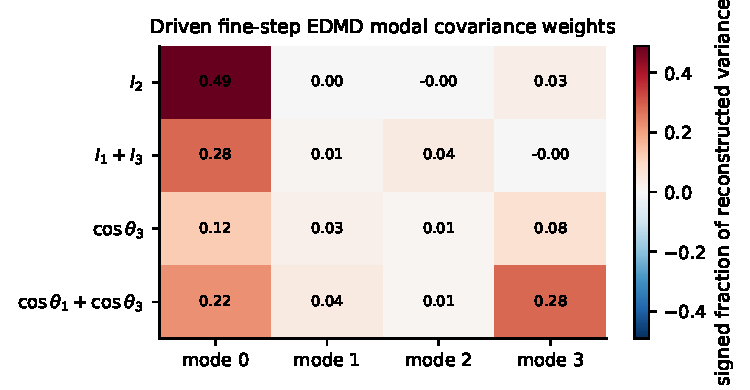
\includegraphics[width=.68\linewidth]{../figures/edmd_observable_weights.pdf}
\caption{Signed modal covariance weights for the first four driven fine-step
reference candidates.  Only mode 0 is finally reportable; the other columns
are diagnostic and must not be read as validated eigenvalues.}
\end{figure}

This pattern is consistent with the autocorrelation plateaus being finite-time
mixtures: $I_2$ has the largest weight on the slow mode and gave the least
negative plateau, whereas the angular observables carry more unresolved faster
weight and gave more negative plateaus.  It does \emph{not} establish the
stronger hypothesis of several distinct, resolved driven slow modes.  The
strict answer to the key question is therefore negative at the present
dictionary and data resolution.

\section{Eigenfunction slices}
Figure~\ref{fig:eigenfunctions} shows the real parts of all fine-timestep modes
that survive the complete gates: the driven and equilibrium leading modes and
the additional equilibrium mode near $-2.86$.  Each row has its own colour
scale, so amplitudes should not be compared between rows.  Numerical values on
the full $81\times81$ grids are saved in
\texttt{analysis/reportable\_eigenfunction\_slices.csv}.

\begin{figure}[h]
\centering
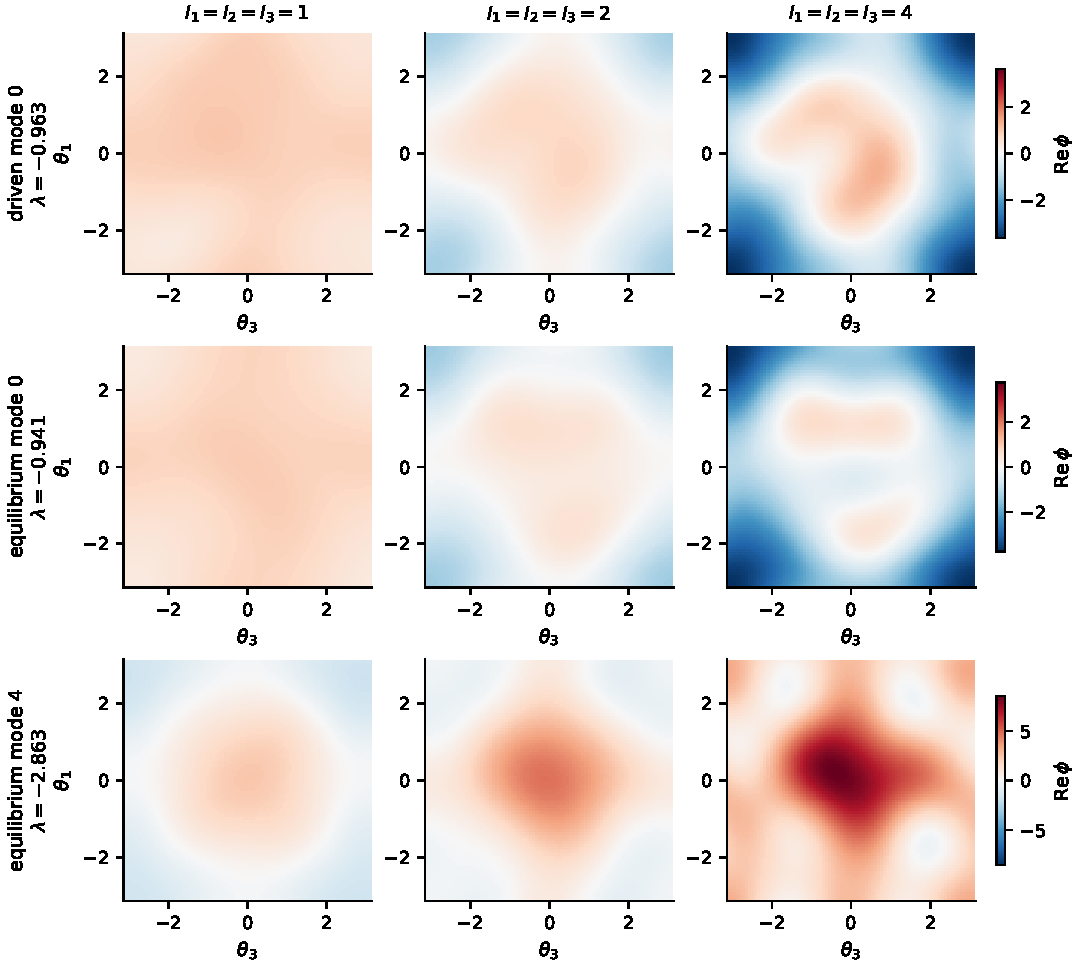
\includegraphics[width=.94\linewidth]{../figures/edmd_reportable_eigenfunctions.pdf}
\caption{EDMD eigenfunction slices in the $(\theta_1,\theta_3)$ plane at equal
actions 1, 2, and 4.}
\label{fig:eigenfunctions}
\end{figure}

\section{Conclusion and claim boundary}
The EDMD computation resolves a robust leading real mode near $-0.95$ in both
bath conditions and both timesteps.  It also resolves a faster equilibrium
mode near $-2.85$.  In the driven case, no second nontrivial rate is both
converged and statistically separated.  The known oscillatory mode is not
recovered under the lag gate.  Accordingly, the defensible claim is:

\begin{quote}
EDMD independently identifies a common leading relaxation rate near $-0.95$
and shows strongly observable-dependent modal weights, consistent with
finite-window contamination of single-observable autocorrelation rates.  It
does not yet resolve a multi-mode driven spectrum or the known oscillatory
pair.
\end{quote}

This is not an exact generator-spectrum proof and not a unique spectral-gap
theorem.

\section{Provenance and raw outputs}
The trajectory simulator source SHA-256 is
\nolinkurl{58c871882f1180701a7aae637a8f4be113315a72fb9d7815562f5fc90faf7976};
the binary SHA-256 is
\nolinkurl{f7cd820bb8f716a8790f688db060259da5657e4f20fa09100546e66efb696b3f}.
The production launch commit is
\texttt{899a5d345a98e4c8d5605a6a5a166a08bb86adcd}.  Base seeds are
2026090801--2026090804 in case order; all 64 deterministic stream seeds per
case are in the original \texttt{metadata.csv} files.  The EDMD protocol was
frozen before spectrum computation, and the analysis source run had SHA-256
\nolinkurl{d4c53270ed902cbcf6692dcc64d7c1f423e40189504d03703c6e4f8cd50cc6ef}.

The exact command was
\begin{verbatim}
python3 run_edmd.py --input ../spectral_gap_controlled_2026-09-07/raw \
  --output analysis
\end{verbatim}
followed by the frozen gate summarizer and figure/audit scripts recorded in
\texttt{provenance/commands.txt}.  All $A$ and $B$ matrices are compressed CSV
files under \texttt{analysis/matrices}; all eigenvalues, 500 replicate-level
bootstrap matches, Gram diagnostics, observable weights, convergence gates,
and eigenfunction grids are CSV files under \texttt{analysis}.  The automated
integrity audit passed 42/42 checks.  SHA-256 values are in
\texttt{provenance/analysis\_outputs.sha256}.

\end{document}
